\documentclass[10pt,letterpaper]{article}

\usepackage[english]{babel}
\usepackage[utf8]{inputenc}

\usepackage{amsmath}
\usepackage{amssymb}
\usepackage{graphicx}
\usepackage{subcaption}
\usepackage{caption}

\usepackage[top=1in, bottom=1in, left=1in, right=1in]{geometry}
\graphicspath{{./imagenes/}}

\begin{document}
	
	\begin{titlepage}
		\centering
		
		{\scshape\LARGE Universidad Nacional Autónoma de México \par}
		
		\vspace{1cm}
		{\scshape\Large Facultad de Ciencias\par}
		\vspace{1.5cm}
		
		\begin{figure}[h]
			\centering
			
\includegraphics[scale=0.15]{logo.png}
		\end{figure}
		
		\vspace{.8 cm}
		
		{\LARGE Práctica 08 \par}
		
		\vspace{0.5cm}
		\large{\itshape{Vianey Aileen Borrás Pablo}} \small{ - 316033619} \\ \vspace{0.3cm}
		\large{\itshape{Kevin Axel Prestegui Ramos}} \small{ - 316201373} \\ \vspace{0.3cm}
		\vfill
		
		\textbf{Arquitectura de Computadoras}\\
		\textbf{Dr. Jorge Luis Ortega Arjona}. \par
		\vspace{0.5cm}
		Fecha de entrega: \textbf{22 de mayo de 2020}.
	\end{titlepage}

	\begin{enumerate}
		
		\item Crear una ALU de 1 bit que realice las siguientes operaciones: AND, OR, Suma,Resta.
		
		\hspace*{0.5cm} Para poder implementar el ALU, ocupamos las puertas AND,OR,NOT y un Multiplexor, recordemos antes las tablas de verdad de cada una de ellas.
		
		\begin{figure}[h!]
			\centering
			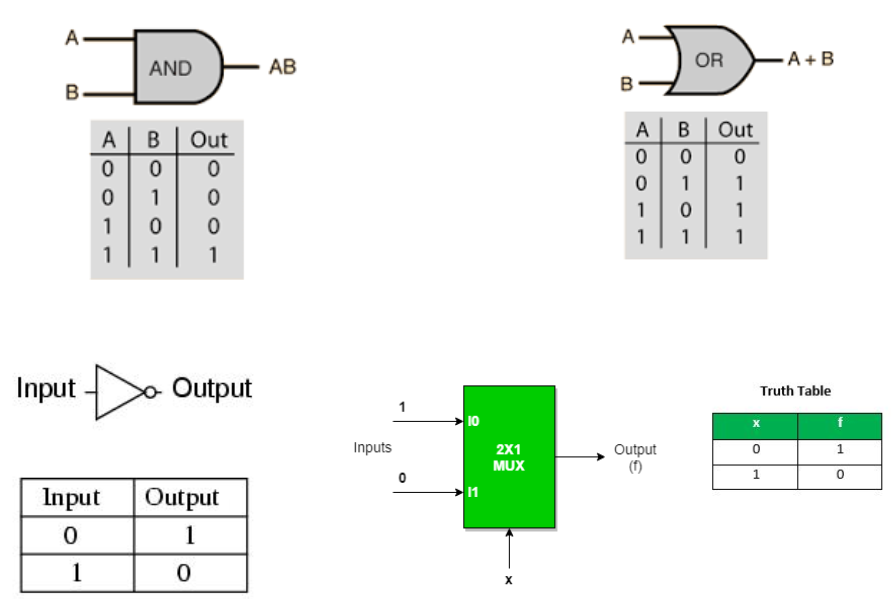
\includegraphics[scale=0.30]{Gates.png}
		\end{figure}
		
		\hspace*{0.5cm} Con ellos podemos construir una ALU de un bit que pueda implementar las operaciones de suma, resta, AND y OR.
		
		\hspace*{0.5cm}Para poder constuir el ALU de 1 bit, seguimos los siguientes pasos:
		
			\begin{itemize}
				
				\item \textbf{Paso 1}\\
				\hspace*{0.5cm} Lo primero que se tiene que hacer es construir una ALU donde solo se pueda llevar a cabo las operaciones lógicas AND y OR. Para esto necesitamos usar ambas puertas lógicas y un multiplexor de 2 a 1 el cual se encargara de decidir que resultados de las operaciones se tiene que mostrar.
				Ver Figura 1 (a).
				
				\item \textbf{Paso 2}\\
				\hspace*{0.5cm} Una vez realizado el paso 1, procedemos a añadir la suma, para ello solo necesitaremos agregar un sumador completo al diseño anterior. Añadimos el circuito que logisim trae para sumas completas el cual tiene dos entradas, un acarreo de entrada (CarryIn) y un acarreo de salida (CarryOut) para la suma actual, esto es en caso de que al momento de procesar la suma suceda un overflow.
				Ver Figura 1 (b).
				
				\item \textbf{Paso 3}\\
				\hspace*{0.5cm} Finalmente añadimos una ultima operación la cual sera la resta. Recordemos que para realizar una resta hacemos uso del complemento a 2 el cual se aplica al segundo valor que entra (B).Usaremos un decodificador el cual estará conectado a otro multiplexor, cuando ingresemos un valor a la entrada B tomara su complemento a 2 sólo en caso de que queramos hacer uso de la resta. Sin embargo aún nos falta agregar un uno extra, recordemos que cuando pasamos un valor a complemento a 2 invertimos los 0 a 1 y los 1 a 0 y sumamos un uno al resultado, esto lo logramos cuando agregamos una constante al acarreo del sumador de logisim mediante el uso de un multiplexor.
				Ver Figura 1 (c).
				
			\end{itemize}
				
			\begin{figure}[h!]	
				\centering	
				\begin{subfigure}{0.35\linewidth}
					\centering
					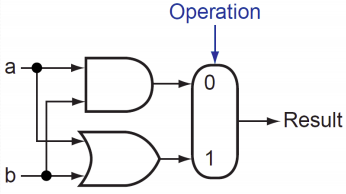
\includegraphics[width=\linewidth]{Paso1.png}
					\caption{Paso 1}				
				\end{subfigure}
				\begin{subfigure}{0.35\linewidth}
				\centering
				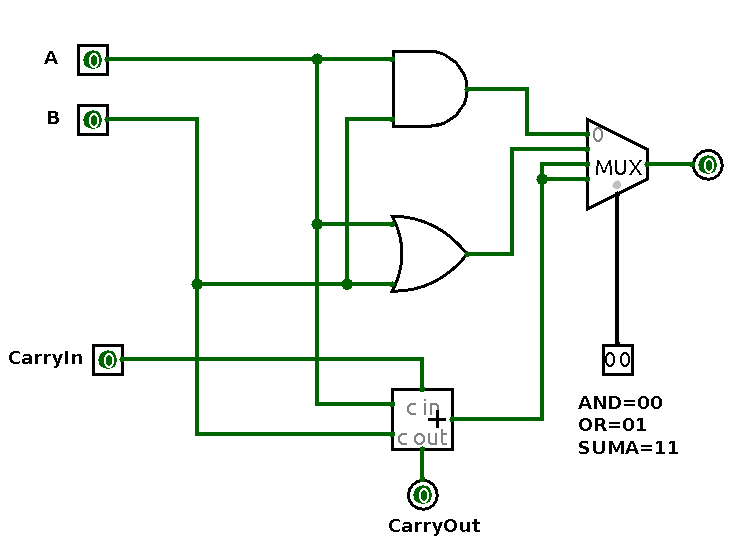
\includegraphics[width=\linewidth]{Paso2}
				\caption{Paso 2}
				\end{subfigure}				
				\begin{subfigure}{0.35\textwidth}
					\centering
					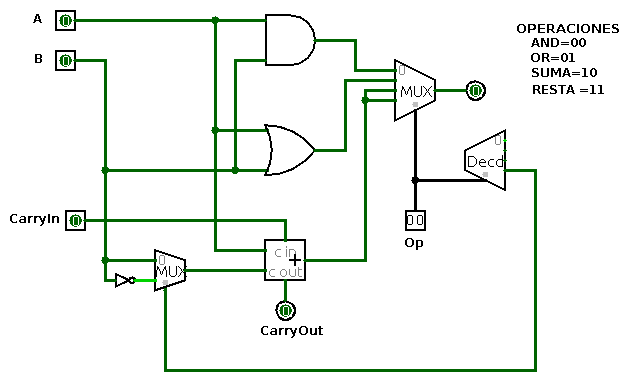
\includegraphics[width=\textwidth]{Paso3}
					\caption{Paso 3}
				\end{subfigure}
			\caption{ALU de 1 bit}
			\end{figure}
		
		\newpage
		
		\item Una ALU de 8 bits reutilizando el ALU de 1 bit.
		
		\hspace*{0.5cm} Para este circuito solo necesitamos repetir ocho veces la ALU de 1 bit, los cuales estarán conectados tanto a las estradas A y B que es por donde pasaremos los valores, cuando queramos realizar la resta, necesitamos obtener el complemento a 2 del valor de B, por lo que añadimos un decodificador el cual se encargara de mandar una señal de activación al acarreo del primer ALU de un bit.
		
		\begin{figure}[h!]
			\centering
			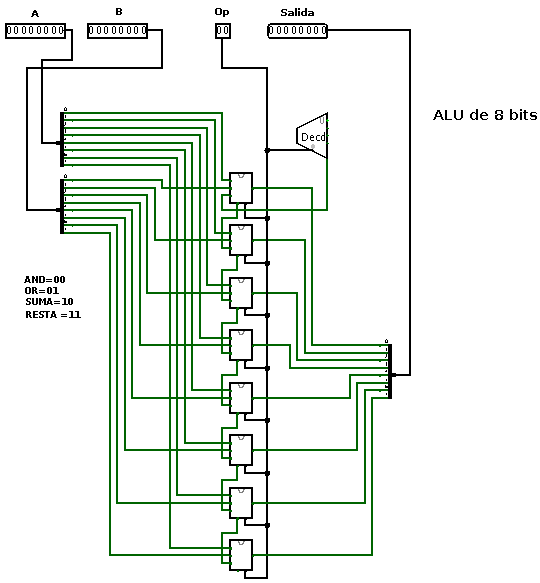
\includegraphics[scale=0.43]{ALUde8bits}
			\caption{ALU de 8 bits}
		\end{figure}
		
		\item ¿Cuántas operaciones más podemos agregar a la ALU? ¿Qué tendríamos que modificar para realizar más operaciones?
		
		\hspace*{0.5cm} Podemos agregar tantas operaciones queramos, algunas de ellas son: multiplicación,división,NOT A, NOT B, XOR, XNOR, NAND,...\\
		\hspace*{0.5cm} Si queremos agregar estas operaciones primero necesitaríamos diseñar por aparte aquellas operaciones que se desean añadir al ALU, asi como se diseño el ALU de 1 bit el cual ocupamos para diseñar el de 8 bits, además necesitamos agregar otro multiplexor donde las combinaciones sean mayor o igual al número de operaciones que tenemos en nuestra ALU.
		
		\item Resta
		
		Ver paso 3 del diseño de una ALU de 1 bit
		
	\end{enumerate}
	
\end{document}